
%%%%%%%%%%%class file
\documentclass{imammb}


%this command gives the journal no. 
%
\jno{dqnxxx}
%%%%%%%%%%%%%%


%%%%%%%%%%%%%%%%%
%call  packages
\usepackage{natbib}
%%%%%%%%%%%%%%

%%%%%%%%%%%%%%%%%%

\usepackage{graphicx}
\usepackage{amsmath,amsthm,bm,mathrsfs}

%%%%%%%%%%%%%%%%%


%%%%%%%%%%%
%this files contains Theorem styles based in IMA JOURNALS
%
\input standard.tex

%%%%%%%%%%%%%


\renewcommand{\theequation}{\thesection.\arabic{equation}}
\numberwithin{equation}{section}
\def\citeasnoun{\cite}
\newcommand{\comment}[1]{}


\begin{document}

%%%%%%%%%%%%%%%%%
\title{Analyzing the propensity for superspreading using finite mixture branching process epidemic models}
\author{ {\sc Suzanne M. O’Regan and John M. Drake}\\[2pt]
Odum School of Ecology, University of Georgia, Athens GA 30602\\[6pt]
{\rm [Received on XX]}\vspace*{6pt}}
\pagestyle{headings}
\markboth{S. M. O'REGAN \& J. M. DRAKE}{\rm SUPERSPREADING USING FINITE MIXTURE BRANCHING PROCESSES}
\maketitle




%\usepackage{xcolor}
%\renewcommand{\arraystretch}{1.5}
%\usepackage{lscape}
%\usepackage{geometry}
%\usepackage{natbib}
%\usepackage{cite}
%\geometry{margin=1in}



\section{Introduction}
Heterogeneity in disease transmission arises frequently in epidemics. Individuals can vary in their ability to transmit infectious agents through biological, behavioral and environmental factors \citep{Lloyd-Smith2005-ma, Althouse2020-dn}. Superspreading events, where one infected individual gives rise to a large number of secondary infections in a single generation, may be the source of most of the secondary cases in a population \citep{Althouse2020-dn}. Contact patterns and social structure may interact with differences in individual infectiousness, giving rise to superspreading events. For example, the first wave of the SARS CoV-2 pandemic was characterized by multiple superspreading events (e.g.\citep{Hamner2020-zt, Adam2020-xk} (Hamner et al. 2020; Illingworth et al. 2021; Adam et al. 2020; Lemieux et al. 2021) ). Understanding the role of superspreading individuals in fuelling transmission in an outbreak is important for epidemic containment. 

%should this be split into multiple paragraphs? e.g contact and behavior examples, biology, environment examples. environment may need to be expanded upon further.
Individual variation in behavior, biology and environment can all induce superspreading transmission patterns. Opportunities for superspreading may arise from heterogeneous contact patterns. For example, \citet{Sneppen2021-mr} characterized contact heterogeneity in SARS CoV-2 transmission by distinguishing between transmission occurring in social networks consisting of mostly regular contacts (e.g., individuals encountered on a daily basis such as those within one’s household) and transmission occurring in large contact networks consisting of individuals encountered infrequently (e.g., encounters in retail stores, bars or public transport). Their modeling showed that individuals whose social network consists of high numbers of infrequently encountered individuals (e.g., retail workers) have a greater diversity of contacts and therefore greater propensity for superspreading than individuals with narrow social networks and few random contacts (e.g., remote workers). Biological factors that increase the probability of successful transmission and the contact rate per infectious individual can also induce superspreading. These include heterogeneities in shedding rate and/or viral load, differences in transmission mode (e.g., aerosol vs. droplet transmission) and symptomatology (asymptomaticity/mild symptoms vs. severe symptoms) \citep{Chen2021-nx, Chen2021-wo}(Illingworth et al. 2021; Chen et al. 2021). For example, if transmission occurs primarily via aerosols, more people can become infected as aerosols travel further and hang for longer in the air, in contrast with droplets that quickly fall to a surface. Frequenting crowded poorly ventilated environments where it is difficult to implement social distancing can also contribute to superspreading transmission, particularly if combined with biological factors (e.g., frequent coughing) or behavioral factors (e.g., refusal to wear a mask in crowded settings). In particular, there is a need to distinguish between heterogeneities in transmission that arise due to supershedding, which is due to biological factors, and superspreading, which arises primarily due to contact patterns \citep{Rock2014-nc}. Much of these heterogeneities are likely to impact the contact process that results in transmission.

%In sum, the probability distribution of the number of secondary infections $N$ depends on just two microlevel processes: a contact process $\{K(x)\}$ leading to infections that each infectious individual independently follows and the infectious period cumulative distribution $F_I(x)$. We note that different specifications of these processes and mixtures can induce the same GW process with mean $R_0$ and offspring distribution of N at the macro-level (Yan 2008).

%In theory for branching processes of epidemics, the cumulative number of contacts with susceptibles leading to infection made by an infectious individual over the course of their infectious period is modelled (e.g., Mode and Sleeman 2000, Yan 2008). A Poisson contact process with intensity $\lambda q$ is typically assumed,  where $\lambda$ is the expected number of contacts per unit time and $q$ is the probability of infection given contact. A Poisson process implies that the time between transmission contacts (exposures leading to infection) is exponentially distributed (Mode and Sleeman 2000, Yan 2008, Diekmann Heesterbeek and Britton 2013) and thus contacts with susceptibles are effectively random. The next consideration is how the infectious period is modelled. For example, in Crump-Mode-Jagers (CMJ) branching processes, which evolve over continuous time, the infectious period for each individual is taken to be a random variable. Various assumptions for the infectious period distribution have been employed including exponential distributions, gamma distributions and log normal distributions (cite). An exponentially distributed infectious period implies that the majority of cases recover rapidly from infection. In contrast, the latter two have a central tendency, which more realistically describes the distribution of the infectious period for many diseases (Keeling and Rohani 2008). Mixing the Poisson contact process with the distribution of the infectious period yields a mixture distribution that describes the number of offspring (cases) per generation (Mode and Sleeman 2000, Yan 2008, Diekmann Heesterbeek and Britton 2013). Conveniently, CMJ processes have an embedded discrete-time Galton-Watson (GW) process that tracks the number of offspring per generation and governs threshold behavior \citep{Mode2000-hp}. It is the offspring distribution arising from a GW process that is typically simulated (e.g. \citep{Lloyd-Smith2005-ma, Kucharski2015-lh, Endo2020-td, Hellewell2020-go})(Lloyd-Smith et al. 2005; Kucharski and Althaus 2015; Endo et al. 2020; Hellewell et al. 2020). Additionally, the theory of GW processes offers many analytical and computational advantages. The number of cases per generation can be simulated easily, the probability of a large outbreak can be calculated and the distribution of transmission chains that go extinct can often be obtained (e.g, \citep{Blumberg2013-xv}).

In theory for branching processes of epidemics, the probability distribution of the number of secondary infections per generation depends on just two microlevel processes: a contact process leading to infections that each infectious individual independently follows and the infectious period cumulative distribution function (Yan 2008). Firstly, the process describing the cumulative number of contacts leading to infection made by an infectious individual with susceptible individuals per unit time is specified (e.g., Mode and Sleeman 2000, Yan 2008). A Poisson contact process with intensity $\lambda q$ is typically assumed, where $\lambda$ is the expected number of contacts per unit time and $q$ is the probability of infection given contact. A Poisson process implies that the time between transmission contacts (exposures leading to infection) is exponentially distributed (Mode and Sleeman 2000, Yan 2008, Diekmann Heesterbeek and Britton 2013) and thus contacts with susceptibles are effectively random. Second, a model for the infectious period is specified. For example, in Crump-Mode-Jagers (CMJ) branching processes, the infectious period for each individual is a continuous random variable. Common assumptions for the infectious period distribution include the exponential distribution, and the gamma distribution. An exponentially distributed infectious period implies that the majority of cases recover rapidly from infection. In contrast, a gamma distribution can be parameterized to have a central tendency, which more realistically describes the distribution of the infectious period for many diseases (Keeling and Rohani 2008). Mixing the Poisson contact process with the distribution of the infectious period yields a mixture distribution that describes the number of offspring (cases) per generation (Mode and Sleeman 2000, Yan 2008, Diekmann Heesterbeek and Britton 2013). Conveniently, CMJ processes have an embedded discrete-time Galton-Watson (GW) process that tracks the number of offspring per generation and governs threshold behavior \citep{Mode2000-hp}. Typically researchers simulate the number of secondary infections per individual in discrete time using an offspring distribution arising from a GW process (e.g. \citep{Lloyd-Smith2005-ma, Kucharski2015-lh, Endo2020-td, Hellewell2020-go})(Lloyd-Smith et al. 2005; Kucharski and Althaus 2015; Endo et al. 2020; Hellewell et al. 2020). Additionally, the theory of GW processes offers many analytical and computational advantages. The number of cases per generation can be simulated easily, the probability of a large outbreak can be calculated and the distribution of transmission chains that go extinct can often be obtained (e.g., \citep{Blumberg2013-xv}).
 
The negative binomial distribution is the most commonly used offspring distribution for modeling superspreading events. Typically the micro-level assumptions of its underlying CMJ process are a Poisson contact process and a gamma-distributed infectious period, with the resulting mixture distribution being negative binomial e.g., \citep{Lloyd-Smith2005-ma}. However, heterogeneous transmission is often characterized by the host population being partitioned into two or more groups, e.g., by social, biological, behavioral or environmental risk structure (Keeling and Rohani 2008, Rock et al. 2014).   Each group has distinct characteristics that affect the distribution of the total number of secondary infections per infected individual belonging to that group. For example, an important aspect of population heterogeneity that is often neglected is the partitioning of the population by average contact rate. Heterogeneity can arise if a certain proportion of the population have high random mixing levels, or if a certain proportion of the population have high shedding rates leading to a higher probability of infecting others or if a certain proportion of the population engage in risky behavior. Models for the distribution of secondary infections that combine heterogeneous transmission patterns with realistic distributions of infection duration are currently lacking.
 
Here we study the effect of the simplest heterogeneous population structure by dividing the population into two groups that are characterized by different average total number of contacts leading to infection per unit time, i.e., two Poisson processes with different intensities. Dividing the population into subpopulations with different transmission rates gives rise to a contact process described by a finite mixture of two Poisson distributions. A finite mixture of negative binomial distributions with the same dispersion parameter arises from mixing the Poisson finite mixture with a gamma distribution for the infectious period. Then a finite mixture of geometric distributions and a finite mixture of Poisson distributions arise as special cases.  To study the stochastic characteristics of transmission at the beginning of an outbreak and the propensity for superspreading events arising from these models, we calculate the mean and variance of the secondary infection distributions, use the generating functions to calculate the probability of a major epidemic when $R_0>1$, and we derive the transmission chain size distributions conditioned on extinction. To understand how these key statistics differ from those generated assuming no contact heterogeneity, we compare the statistics obtained from the mixture distributions with those generated by a negative binomial distribution with the same mean and dispersion parameter in the number of cases.  %We study three finite mixtures: a model with transmission heterogeneity only (a finite mixture of two Poisson distributions) and two models with heterogeneities in transmission patterns and infection duration (finite mixtures of two negative binomial distributions and two geometric distributions).

%do they have the same variance? I think not, because p varies. The bit that is different is G''(N)
 
Long-tailed secondary infection distributions induce greater variability in transmission chain size, which can be characterized by larger probability of observing no secondary infections, smaller probability of major epidemics, larger coefficient of variation in the number of secondary infections and greater probabilities of observing a chain larger than a given size than for Poisson epidemics \citep{Althouse2020-dn}. To examine implications for superspreading and containment, we study the effect of decreasing $R_0$ in three ways. First we alter the heterogeneous structure of the population by examining the effect of varying the transmission heterogeneity ratio $p$. We reduce the proportion of individuals with high transmission rate, which is equivalent to decreasing the proportion $p$ of the population that do not comply with stay-at-home orders or with face covering mandates, do not self-isolate when sick or decreasing the proportion of the population with high probability of transmission through viral load or shedding rate. Next we decrease the average number of additional successful contacts per generation in the superspreading cohort while keeping it fixed in the remainder, which may be viewed as decreasing their intensity of interactions (e.g., by changing the working environment). Third, we decrease baseline transmission rate in both groups simultaneously e.g., both groups wear face coverings. %alter risk structure
 
%In summary, our key questions are:
%\begin{itemize}
%    \item Does the mechanistic addition of population structure induce qualitatively different outbreak patterns from a standard negative binomial superspreading model with mean $R_0$ and dispersion parameter $k$ assuming $R_0>1$? 
%\item How does decreasing the level of superspreading by a) changing the population structure e.g., by shifting the contact structure away from opportunistic encounters/aerosol transmission and towards regular contacts/direct contact transmission, and b) decreasing the average number of successful contacts in the superspreading cohort affect heterogeneity in outbreak patterns, and what are the implications for containment?
%\end{itemize}

Our work shows that the mechanistic addition of population structure induces qualitatively different outbreak patterns from a standard negative binomial superspreading model with mean $R_0$ and dispersion parameter $k$. We show that the critical threshold for containment is different depending on whether superspreaders only are targeted or both cohorts are targeted, and which of these strategies is the most effective is context-dependent. 

\section{Methods}
%high level summary of approach
%need to introduce the base model for superspreading

\subsection{Review of standard superspreading model}

%also standard superspreading model can be derived by assuming a Poisson contact process, gamma distributed infectious period and their mixture is negative binomial. 
%I don't want to be heavily critical of the model either. just want to examine how exactly superspreading arises, and deriving a more mechanistic model. 
We begin by studying the derivation of the standard superspreading model in Lloyd-Smith et al. 2005 and its microlevel processes. 
Each individual has a reproductive number. Individual reproductive numbers are gamma-distributed due to mixing gamma distributed infectious period with constant contact rate per infectious individual. Demographic stochasticity in the number of secondary infections per individual is Poisson distributed. Integrating over all possible individual reproduction numbers yields a negative binomial model with mean $R_0$ and dispersion $k$. Alternatively the model can be derived by assuming a Poisson contact process, gamma-distributed infectious period and their mixture is negative binomial (e.g., Heesterbeek, Yan) . In both of these formulations of the standard model, all heterogeneity is due to the infectious period only. The model does not capture heterogeneity in population structure that could additionally induce superspreading (e.g., processes listed in Table 1). Here we aim to examine the micro-level processes that induce superspreading transmission, and to use them to derive a more mechanistic model. 

%criticism: too coarse?
%moreover the standard model assumes that the superspreading comes from the gamma distributed infectious period only and the mixing with poisson is due to the coarse assumption of demographic stochasticity (in what?) or it comes from individual reproduction numbers that are gamma distributed. and what is an individual reproduction number? individual contact rate * individual inf period. The inf period being drawn from gamma....but they assume everyone in the population has the same contact rate (i.e. it is not an rv) 
%neg binom macroscale (generation) Here we look at microscale processes at the individual level 

%gamma distribution with small k: most people recover quickly, but a few take extremely long time to recover. 

%mechanistic derivation? the standard model for superspreading is the negative binomial with mean R0 and dispersion k. There are a couple of things I can see. For example Lloyd Smith et al used a neg binom model for superspreading by arguing that individual reproductive numbers were gamma distributed with mean R0 and dispersion parameter k and demographic stochasticity was Poisson distributed. The resulting Poisson-gamma mixture distribution is a negative binomial. On the other hand, a negative binomial can be derived by gamma distributed infectious period with mean 1/gamma and CV 1/k and Poisson contact process with intesnity beta. That model would have the superspreading component captured by the dispersion parameter - disadvangtage since it suggests 

%see Nishiura
%want to also argue our model gives rise to a gW branching process that wesimulate

\subsection{Mechanistic superspreading model}

%different microlevel processes can lead to superspreading at the macrolevel. %To model superspreading, we need to consider what happens on the microlevel

 [High level overview of modeling approach]
 
 %should i define microlevel processes before this paragraph? 
We distinguish between superspreading and regular transmission.  Infectious individuals may have superspreading transmission characteristics or they may have non-superspreading (i.e., regular) transmission characteristics. Table 1 summarizes examples of micro-level processes that may underpin heterogeneous transmission in a population. Sources of heterogeneity can either partition the population into distinct groups (e.g., occupation) or they can be continuous (e.g., infectious period) and may either affect the contact process or the duration of infectiousness. Here we develop a branching process model that combines both binary and continuous sources of heterogeneity. Specifically, we develop a model of a Crump-Mode-Jagers (CMJ) continuous-time branching process that accounts for micro-level transmission. Following Yan (2008), at the micro-scale, the CMJ process assumes that infectious individuals have independently and identically distributed infectious period (generation time), in which individuals produce secondary infections according to a contact process $\{K(x)\}$. The generation time and contact processes are independent, and at the end of the generation time, the infectious individual produces a random number $N$ of secondary infections. Embedded within the CMJ branching process, there is a macro-level discrete-time Galton-Watson (GW) branching process that we use to derive key statistics such as the basic reproduction number, i.e., the mean value of the GW process $R_0=E[N]$ and the probability of extinction (Mode and Sleeman 2000, Yan 2008). 

%high level overview of superspreading models
%Heesterbeek: expected number of contacts per unit time with other individuals

%we note as well that these sources of heterogeneity can affect either the contact process or the infectious period. 
%high level summary: disease transmission consists of a mixture of two stochastic processes: contact and infectious period. 
%follow Yan 2008 and Mode and Sleeman



\begin{table}[b!] %T2
\tblcaptionnotes{Mechanisms for heterogeneous transmission from infectious individuals to susceptible individuals. Sources of heterogeneity at the micro-level can be binary (i.e., processes that partition individuals into disjoint groups) or continuous (e.g., duration of symptoms, infectiousness)}
{\mbox{\tabcolsep=10pt\begin{tabular}{@{}cc@{}}
\tblhead{Source of heterogeneity & Factor \\[-11pt]}\\[-9.5pt]
Micro-level binary &  \\[3pt]
Proximity to susceptible individuals (remote worker vs. healthcare worker) 
& Environmental \\[3pt]
Transmission mode (e.g., aerosol vs. droplet transmission)   &Biological  \\[3pt]
Symptomatology (e.g. shedding at high rates vs. low rates) &  Biological
\\[3pt]
Compliance behaviors (e.g., self-isolation when sick vs. no self isolation)   &Behavioral \\[3pt]
Susceptibility (e.g., having underlying health conditions or not, smoker/non-smoker) & Biological/Behavioral\\[3pt]
Micro-level continuous &  \\[3pt]
Symptomatology (infectiousness affecting probability of infection given contact) & Biological \\[3pt]
 Symptomatology  (severe longlasting symptoms that correlate with infection duration)& Biological \\[-9pt] \lastline
\end{tabular}
\label{Neigs2}
}}{}\vspace*{-2pt}%leave footnote space blank, e.g. $^a$ Iteration counts obtained with the ideal preconditioner are
%listed in columns 2--3 of Table 2\\$^b$ The negative eigenvalues
%of the preconditioned saddle point system.
\end{table}

To account for population risk structure (Table 1), we begin by dividing the population into two disjoint classes: a fraction $p$ belonging to a superspreading cohort and the remainder $1-p$ are members of a regular cohort. The superspreading cohort could be characterized by frequenting a risky environment (e.g., working in a densely populated environment), irregular biology (for example, having a tendency for super-shedding) or risk taking behavior. The regular cohort does not have environmental, behavioral or biological attributes that may characterize superspreading or supershedding. Examples of settings with a strict partition of the population  include workplaces (e.g. a meat factory with workers on the floor and office workers, with a public space such as a cafeteria where mixing of both cohorts occurs, schools with classroom bubbles (teachers may have lots of contacts because they teach numerous classroom cohorts whereas students only contact nearest neighbours in the classroom) or binary partitioning of a closed population according to a categorical variable that affects susceptibility or infectiousness (for example, characterizing patients in a care home according to whether they smoke (a risky behavior) or not). We assume the two cohorts contact others according to Poisson processes with different intensities, with the superspreading cohort having a higher average successful contact rate where they spread infection to susceptible individuals than the regular cohort. The average contact intensity leading to transmission is the product of the average contact rate and the probability of transmission given contact. We denote this product by $\beta$ in the regular cohort and by $\beta^S$ in the superspreading cohort. We assume mean superspreading contact intensity $\beta^S $ is comprised of mean regular contact rate $\beta$ and mean additional transmission contact rate $\tilde{\delta}$,
\begin{equation}\label{eqn:R0Adel}
   \beta^S = \beta +\tilde{\delta}, \quad \tilde{\delta} >0.  
\end{equation}
Letting $C$ be a random variable denoting the cumulative number of transmission contacts (contacts that infect susceptibles) by time $x$,  a finite mixture of Poisson distributions with probability mass function %strictly speaking this is lambda q and lambda^s q, with q binomial (either infected or not). mixture of Poisson and binomial is Poisson (Heesterbeek 2013)
%this pmf is the pmf conditional on the value of x. 
%advantage of mode and sleeman approach is that it makes the connection with embedded GW process explicit. easier to argue we simulate by generation time. 
\begin{equation}\label{eqn:contactpmf}
  P(C=c)=  p \frac{(\beta^S x)^c}{c!} e^{-\beta^S x} +(1-p)\frac{(\beta x)^c }{c!} e^{-\beta x}
\end{equation}
and probability generating function
\begin{equation}\label{eqn:contactpgf}
    G(s,x) = p \exp \left ( \beta^S x (s-1) \right)  + (1-p) \exp  \left (\beta x (s-1)\right), \quad s \in [0,1]
\end{equation}
describing the stochastic contact process $\{C(x): x \in [0, \infty)\}$ in the population. The contact process is a counting process that stops when the infectious period of an infective ends. The stopping time is defined by the length of the infectious period $T_I$, itself a random variable. Here we assume that in both groups, following \citet{Anderson, Britton} the infectious period is gamma distributed with mean $1/\gamma$ and coefficient of variation $1/\sqrt{k}$ with probability density function
\begin{equation}\label{eqn:gammapdf}
f_I(x) = \frac{(\gamma k)^k}{\Gamma(k)} x^{k-1}e^{-k \gamma x}
\end{equation}
and cumulative distribution function $P(T_I \leq x) = \int_0^x f_I(x) dx$. Here $k$ is a positive real number and $\Gamma(k)$ denotes the gamma function. The gamma distribution is flexible in that it allows for heavily right-skewed distributions (i.e., $k<1$), and distributions with a central tendency ($k>1$). If $k=1$, the distribution becomes the exponential distribution. Infectious period distributions with a central tendency about the mean are often more realistic \citep{Lloyd2001, Wearing2005, Keeling2008-sh} than right-skewed distributions, which assume that most individuals have recovery times that are much shorter than the mean. However, strongly right-skewed distributions (i.e., $k<1$) capture the property of there being a small proportion of individuals in the population with extremely long infectious period, who could therefore make many contacts leading to transmission over the course of being infected.

%here we make the argument that derives the probability generating function for the number of secondary infections. 
%should I put in the argument where N(x) = K(x) x<Ti, K(T_I) x>= T_i for fixed x the number of secondary infections is G_N(s,x)
To find the probability distribution for the cumulative number of transmission contacts generated by an infectious individual throughout its entire infectious period (i.e., the number of secondary infections per infectious individual per generation $N = 0, 1,2, \dots$) following \citet{Mode2000-hp} and \citet{Yan2008}, the expression for the probability generating function is
\begin{align}\label{eqn:mixturepgf}
    G_N(s) &= \sum_{j=0}^{\infty} s^j P(N=j) \notag \\ &= \int_0^{\infty} G(s,x) f_I(x) dx \notag \\ &= \int_0^\infty \left (p e^{\beta^S x (s-1)}+(1-p)e^{\beta x (s-1)} \right) \frac{(\gamma k)^k}{\Gamma(k)} x^{k-1}e^{-k \gamma x} dx.
\end{align}
Letting $\beta /\gamma = R_0^R$ and $\beta^S /\gamma = R_0^S$, evaluating the integral above yields %do I need more info on the integration here? eg gamma functions. See heesterbeek
\begin{align}\label{eqn:nbinommixpgf}
    G_N(s) &=  \frac{p(\gamma k)^k}{(\gamma k + \beta^S(1-s))^k} +   \frac{(1-p)(\gamma k)^k}{(\gamma k + \beta(1-s))^k}\notag  \notag \\ &=  \frac{p}{(1 + \frac{\beta^S}{\gamma k}(1-s))^k} +   \frac{(1-p)}{(1 + \frac{\beta}{\gamma k}(1-s))^k} \notag \\&=  \frac{p}{(1 + \frac{R_0^S}{k}(1-s))^k} +   \frac{(1-p)}{(1 + \frac{R_0^R}{k}(1-s))^k}. 
\end{align}
Equation \eqref{eqn:nbinommixpgf} describes the macro-level Galton-Watson discrete time branching process embedded in the continuous-time Crump-Mode-Jagers branching process at the micro-scale.
We note that different microscale processes can induce the same GW process at the macro-level (Yan 2008). %Different mixtures of contact processes with the distribution of the infectious period can yield the same probability distribution for the number of secondary infections and same $R_0$. 
The basic reproduction number $R_0$ of the mixture branching process (\eqref{eqn:nbinommixpgf}), i.e., the mean number of secondary infections per infectious individual per generation, is  
%\beta^S p k (\gamma k)^k (\gamma k + \beta^S(1-s))^{-k-1} + \beta (1-p) k (\gamma k)^k (\gamma k + \beta (1-s))^{-k-1}
%\beta^S p k (\gamma k)^k (\gamma k )^{-k-1} + \beta (1-p) k (\gamma k)^k (\gamma k )^{-k-1}
%\beta^S p k (\gamma k )^{-1} + \beta (1-p) k  (\gamma k )^{-1}
\begin{equation}\label{eqn:R0}
   R_0= G_N'(1) = p\frac{ \beta^S }{\gamma } +(1-p)\frac{ \beta }  {\gamma  } = p R_0^S + (1-p) R_0^R.%\frac{p(\gamma k)^k}{(\gamma k + \beta^S(1-s))^k} +   \frac{(1-p)(\gamma k)^k}{(\gamma k + \beta(1-s))^k}.
\end{equation}
Evaluating $\frac{1}{j!} \frac{d^j}{ds^j} G_N(0) |_{s=0}$ $j=0,1,2\dots$ yields the probability mass function for the number of secondary infections with parameters $p$, $k$, $R_0^S$ and $R_0^R$,
\begin{equation}\label{eqn:nbinommixpmf}
    P(N=j) =  \frac{\Gamma(j+k)}{j! \Gamma (k)} \left [ p \left(\frac{k}{k+R_0^S} \right)^{k}\left (\frac{R_0^S}{k+R_0^S} \right )^j+ (1-p) \left(\frac{k}{k+R_0^R} \right)^{k}\left (\frac{R_0^R}{k+R_0^R} \right )^j \right ].
\end{equation}
%%this could be done via generating functions or the pdfs themselves. 
%say this is a finite mixture of negative binomials
Equation \eqref{eqn:nbinommixpmf} is a finite mixture of negative binomial distributions that combines regular transmission and superspreading. %together with a realistic distribution for the infectious period
The model is flexible in that it allows for a variety of infectious histories including having extremely high risk of superspreading transmission to others (e.g., high contact rate and long infectious period), high risk of superspreading transmission to others (e.g., high contact rate and fast recovery rate), moderate risk of being a superspreader (e.g., low contact rate and long infectious period) and being characterized by regular transmission (e.g., low contact rate and fast recovery rate). Therefore, model \eqref{eqn:nbinommixpmf} for the offspring distribution more accurately captures a spectrum of infectious histories than the standard negative binomial model with mean $R_0$ and dispersion parameter $k$. 

To examine the influence of having two contact processes with different intensities in the mixture model compared with having just one on the probability distribution, we compare the probability mass functions of the the mixture model \eqref{eqn:nbinommixpmf} with the standard (base) model with same $R_0$ and dispersion parameter $k$ in Figure \ref{fig:pmf}. The probability of an infectious individual producing no secondary infections ($P(N=0)$) is higher in the mixture models than the base model for all values of $k$. As $k$ increases, the level of heterogeneity declines in that $P(N=0)$ declines in both models, but the base model has a greater central tendency than the mixture model. In sum, there are visible differences in the probability mass functions of both models, and we conclude that having a mixture of two contact processes substantially affects the probability mass function. 

%Even though the evolution of an epidemic in continuous time may be
%accounted for in a one-type CMJ-process, all such processes have a
%discrete time BGW-process embedded in them.
%In these branching processes, there is an embedded Galton–Watson branching
%process to track the generations. The basic reproduction number corresponds
%to the mean value of this embedded Galton–Watson branching process
%with R0 = E[N].
%Crump–Mode–Jagers (CMJ) processes. Infected individuals have independently
%and arbitrarily distributed generation time TG. Throughout the
%generation time, each individual produces secondary infections according
%to a counting process {K(x)}. Different individuals follow the same counting
%process. It is assumed that the generation time TG and {K(x)} are
%independent. By the end of the generation time, an infected individual
%produces a random number of N secondary infections.


%moreover the standard model assumes that the superspreading comes from the gamma distributed infectious period only and the mixing with poisson is due to the coarse assumption of demographic stochasticity (in what?) or it comes from individual reproduction numbers that are gamma distributed. and what is an individual reproduction number? individual contact rate * individual inf period. The inf period being drawn from gamma....but i think they assume everyone in the population has the same contact rate (i.e. it is not an rv) 
%neg binom macroscale (generation) Here we look at microscale processes at the individual level 

%need to mention GW process. 
%We note that the tendency for superspreading is captured in the contact process alone.  not necessarility
%compare pmfs of negative binomial and mixture. Should negative binomial be defined above? 
%eps or pdf??
\begin{figure}[!t] %F1
\centering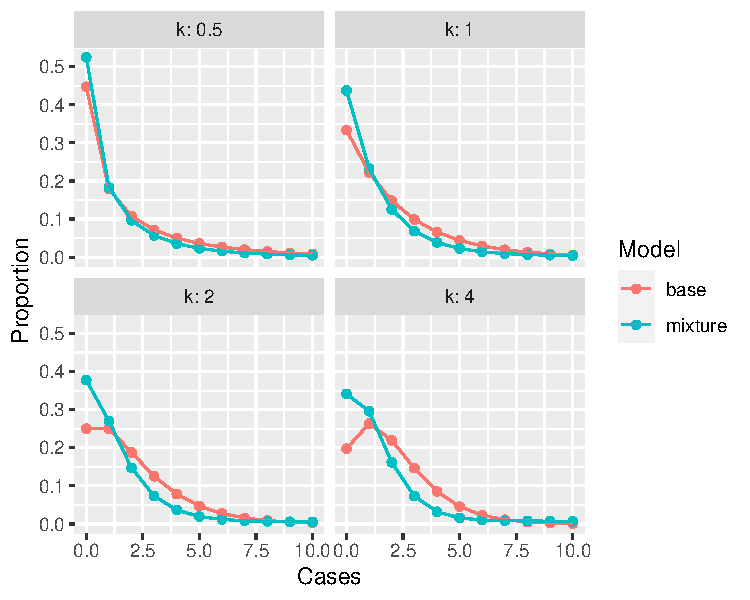
\includegraphics {Figure1.pdf}
\caption{Probability mass functions of the mixture model ($R_0^D=1.1$, $p=0.1$, additional contacts $\delta =9$) compared with those of base model with the same $R_0$ and dispersion parameter $k$. The mean number of secondary infections for both models is $R_0 =2$. For the mixture models, the probability of no secondary infections is always greater than the negative binomial model with the same $R_0$ and $k$. As $k$ increases there is a greater central tendency in the number of secondary infections in the base model.  }
\label{fig:pmf}\vspace*{-9pt}
\end{figure}

%%where does base model go?

%our model shows we have a finite linear mixture of two negative binomial processes with different means but the same dispersion parameter k

\subsection{Statistics} %does this need a subsection
[overview]
%need to define R0 in terms of p and delta. 
Noting that $R_0^R = \beta/\gamma$,  we can rewrite $R_0^S$ in terms of $R_0^R$,
\begin{equation}
R_0^S = \frac{\beta + \tilde{\delta}}{\gamma} = \frac{\beta}{\gamma} + \frac{ \tilde{\delta}}{\gamma} = R_0^R + \delta. 
\end{equation}
Rewriting the basic reproduction number $R_0$ in terms of $\delta$, the expression for the average number of secondary infections due to additional contacts $\tilde{\delta}$ simplifies to 
\begin{equation}\label{eqn:R0delta}
R_0 = R_0^R + p \delta,
\end{equation}
which lies between $R_0^R$ and $R_0^S$ if $0<p<1$. 
% do I need formal definition of R0?
The variance of the number of secondary infections according to the mixture model is %P146 of notes
\begin{equation}\label{eqn:variance}
V(N) = G_N''(1) + G_N'(1) -  (G_N'(1))^2= R_0^R + \frac{(R_0^R)^2}{k} + p \delta \left [ (1+ \delta(1-p) + \frac{2 R_0^R + \delta}{k} \right ]. 
\end{equation}
If $p=0$, then $V(N) = R_0^R + (R_0^R)^2/k$ and if $p=1$, $V(N) = R_0^S + (R_0^S)^2/k$, i.e., equation \eqref{eqn:variance} lies between the two extremes if $0<p<1$. The variance is an increasing function of $R_0^R$ and an increasing function of $\delta$ provided $0<p<1$. However $V(N)$ is a quadratic function of $p$, and it is increasing if $0\leq p \leq 1/2$.

%Heesterbeek: when during a time interval of length deltaT contacts are made according to a Poisson process with rate c, the number of contacts follows the Poisson distribution with mean parameter c deltaT. When contacts lead to successful transmission the number of 'successful' contacts is again Poisson distributed with mean parameter p c deltaT. 

%in other words intensity (rate per unit time) is a random variable with 2 values beta and beta^S with probability (1-p) and p respectively
%%finish this section with figure 1. Follow up with statistics, then probability of extinction 
\comment{
\begin{align*}
P(5 \text{ secondary infections }) &= P( \text{ 5 secondary infections from infectious individual in superspreading cohort}) \\&\text{ or } P( \text{ 5 secondary infections from infectious individual in regular cohort })\\
&=P(\text{choosing regular infectious individ})P(5 \text{ infections conditional on regular infectious individ})\\ &\text{or } P(\text{superspreading})P(5 \text{infections conditional on being from superspreading cohort}), 
\end{align*}
or expressed mathematically as,
\begin{align*}
    P(I=5) &=(1-p) P(I=5|\text{regular}) +p P(I=5|\text{superspreading}) \\
     &=p P(T=5|\mathcal{V}=\beta^D) +(1-p) P(T=5|\mathcal{V}=\beta^A)\\
     &=p \frac{(\beta^D)^5}{5!} e^{-\beta^D} +(1-p)\frac{(\beta^A)^5}{5!} e^{-\beta^A}.
\end{align*}
}
%mathematical derivation of model, including integrating over infectious period, and dividing to express things in terms of individual R0

 %We assume the number of successful contacts per individual per unit time leading to transmission over the course of their infectious period is Poisson distributed. However the number of transmission events per individual depends on whether they have low contact rate (i.e, close contact transmission) or high contact rate (i.e,  superspreading or aerosol transmission) . We assume $p$\% of transmission events occur through close contact, and $(1-p)$\% of transmission events occur via superspreading.
%the number of people they infect (their cumaltive sucessful contacts) depends on their behavioral, bilologixal and environmental characteristics
%differential patterns of mixing
%separating infectious individuals by their contact process. 
%We partition individuals by their successful contact rate


%Table 1?
%, e.g., high pathogen load and release


%- Model assumptions and derivation - does pgf go here? 
%- Figure 1: comparison of probability mass functions for standard and mixture models for various values of $k$
%- To study X, we calculated the following summary statistics. formulas for mean, variance, CV of number of secondary infections 
%\subsection{Statistics}

\subsection{Probability of extinction if $R_0>1$}
To calculate the probability of the mixture branching process becoming extinct, we numerically solve the following equation for the smallest root $s^*$, 
\begin{equation}
      s = G_N(s) =  \frac{p}{(1 + \frac{R_0^S}{k}(1-s))^k} +   \frac{(1-p)}{(1 + \frac{R_0^R}{k}(1-s))^k}. 
\end{equation}
When $R_0<1$, then $s^* = 1$ and a major outbreak cannot occur. If $R_0>1$, either there is a small outbreak that dies out with probability $s^*$ or the number of cases take off, becoming a major outbreak with probability $1-s^*$. If there is a small outbreak, the observed branching process will be the same as that from that arising from a different reproduction number $R_0^* = G_N'(s^*)<1$. (Yan 2008) %another other references? e.g. Nishiura? 



%equation for probability of extinction
% meaning of $R_0^*$ when $R_0>1$

\subsection{Chain size distribution}

To quantify transmission chains, we need the chain size distribution. To derive it, we follow the method in \citet{Blumberg2013-xv}. 

%Derivation
%Figure 2: comparison of chain size distributions for standard and mixture models for various values of $k$
%summary statistics for transmission chains - can use the distirubion to calculate the cumulative probability of observing a small chain
%mean chain size conditioned on extinction 
%variance of chain size conditioned on extinction 

%where does control activities thresholds go?
%what journal to target??

\subsection{Numerical analysis} %studies (assuming $R_0$ > 1)
%How statistics vary with $p$, $\delta$ and $k$, keeping $R_0$ fixed, for the baseline and mixture models (compare the degree of heterogeneity in outbreak patterns)
%Effect of control activities on outbreak patterns: decrease $R_0^D$, $p$ and $\delta$ by factor $1-c$ and study their effect on variance to mean ratio and probability of extinction (which control activity induces greatest probability of extinction for a given level of control effort below the threshold (assuming the threshold for all activities is the same) and do patterns become more heterogeneous as epidemic control is applied?)


\section{Results}
% Figure 3: Coefficient of variation of distribution of secondary infections
% Figure 4: Probability of major outbreak
%Figure 5: Probability of observing a transmission chain of size <= 10
%Figure 6: CV chain size
%Figure 7: Effect of control activities: Control vs. Variance to mean ratio of distribution of secondary infections and  control vs. probability of extinction

\section{Discussion}


 








\bibliographystyle{amnat}
\bibliography{paperpile}
\end{document}
